\part{Metodologia}

\chapter[Metodologia]{Metodologia}

Este capítulo é destinado à apresentar toda a metodologia aplicada a esta
pesquisa. Vale ressaltar que a metodologia proposta nesta pesquisa está sendo
baseada na definição proposta por Silva e Menezes, que afirmam que toda pesquisa
tem como objetivo encontrar respostas para hipóteses propostas
\cite{da2005metodologia}

Com o intuito de classificar a pesquisa sendo desevolvida, observou-se que a
mesma se enquadra como aplicada, quantitativa, exploratória, bibliográfica e
experimental \cite{da2005metodologia}.


\section{Trabalhos relacionados}

Durante a pesquisa deste trabalho, encontrou-se alguns trabalhos que também estudam recomendação baseada em contexto, sendo o tempo um dos
principais atributos do contexto. Em \cite{lee2008time}, o tempo é usado para gerar avaliação implícita para um histórico de
compras de diversos usuários. Tal abordagem foi comparada com um modelo de recomendação colaborativa tradicional, usando avaliação explícita dos usuários,
sem considerar o tempo. Segundo a pesquisa, percebeu-se um aumento de precisão quando o tempo foi usado para gerar a matriz de recomendação.

Outra pesquida relacionada foi a de \cite{ding2005time}. Nesta pesquisa, um
sistema de recomendação colaborativo sensível ao tempo foi criado. O sistema proposto usava uma função de
decaimento exponencial para priorizar itens recentemente avaliados e diminuir o peso de itens avaliados a mais tempo na recomendação. Quando comparado a um sistema de
recomendação colaborativa clássico, percebeu-se um aumento de acurácia para o recomendador sensível ao tempo.

Além de comparação de sistema de recomendação, foi também encontrado um trabalho que propõe um modelo diferente do clássico uso do tempo em recomendação, como o usado em
\cite{ding2005time}. Este modelo foi proposto no artigo de \cite{basile2015modeling}, onde basicamente itens mais antigos não tem seu peso puramente descartado, e sim caso
seu conteúdo seja diferente dos novos itens sendo recomendados. Baseado nos testes realizados, percebeu-se que criar o modelo de usuário dessa forma apresenta vantagens sobre
a forma mais padrão de se usar o tempo para recomendação. Entretanto, o trabalho ainda precisa ser testado em bancos de dados de maior escala para poder aferir melhor seus
resultados

Por fim, um famoso trabalho que usa o contexto de tempo para recomendação se dá na pesquisa \cite{koren2010collaborative}, que apresenta o modelo de recomendação vencedor
do concurso criado pelo Netflix para aumentar a acurácia de suas recomendações de filme. A pesquisa citada usa como diferencial a análise do tempo da avaliação dos filmes
realizados pelos usuários em um modelo similar a pesquisa de \cite{basile2015modeling}


\section{Planejamento da pesquisa}

Tendo como base os conceitos de recomendação apresentados e a forma dinâmica com
que usuários instalam e usam novos pacotes em seus próprios sistemas, esta
pesquisa visa então responder a seguinte questão problema:

\begin{center}
\textit{É possível melhorar a recomendação baseada em conteúdo de pacotes para
usuários de sistemas GNU/Linux levando em consideração o contexto de uso dos pacotes já instalados ?}
\end{center}

\subsection{Hipóteses} \label{sec:hipoteses}

Considerando a questão problema definida, as seguintes hipóteses foram definidas
como forma de validação:

\begin{itemize} \item \textit{\textbf{h1:  Ao aumentar o peso de pacotes
recentemente usados no sistema, o perfil do usuário gerado será mais preciso,
ocasionando assim uma recomendação mais apropriada.}} Ao usar o tempo de uso dos
pacotes no sistema, e priorizar os pacotes mais recentemente usados na criação
do perfil, acredita-se que a mesma irá produzir um perfil mais
consistente do usuário, gerando assim recomendações mais efetivas.\item
\textit{\textbf{h2: Uma abordagem por aprendizado de máquina irá se comportar melhor
        que uma determinística para o problema proposto}}
Considerando os dados presentes em pacotes Debian que podem ser
usados para prover a recomendação, pode-se entender que o uso de uma abordagem
por aprendizado de máquina irá prover melhores resultados, devido a possível
complexidade dos relacionamentos entre os atribuitos dos pacotes.
\end{itemize}

\subsection{Seleção do projeto}

Para validar as hipóteses levantadas, faz-se necessário escolher um projeto
um projeto software livre que implemente um sistema de recomendação de pacotes
para sistemas GNU/Linux e que não use nenhuma informação de contexto em suas
recomendações, de forma a permitir a comparação das abordagens propostas com as
já implementadas pelo projeto.

\subsubsection{Descrição do projeto selecionado}

O projeto selecionado que atendia os requisitos propostos para a pesquisa foi o AppRecommender,
um sistema de recomendação de aplicativos GNU/Linux, cuja principal característica é recomendar aplicações,
onde “dada a lista de programas instalados em determinado sistema, o recomendador retorna uma lista de aplicativos
sugeridos, que supostamente são aplicativos de potencial interesse para os usuários daquele sistema”
\cite{araujo2011apprecommender}.

O AppRecommender possui três categorias para estratégias de recomendação, onde cada
estratégia é uma forma diferente de se obter uma lista de aplicativos sugeridos
através de uma lista de pacotes instalados no sistema, essas categorias de estratégias
são: Baseadas em conteúdo, colaborativas, e híbridas. Segue abaixo as especificações
de cada categoria de estratégia:

\begin{itemize}
    \item \textit{\textbf{Baseadas em conteúdo:}} Esse tipo de categoria de estratégia
        visa montar um perfil de usuário através da lista dos pacotes instalados no sistema,
        onde esse perfil é uma lista composta por tags ou descrições de pacotes que são
        definidas pelo algoritmo de estratégia escolhida, através dessa lista a base de dados
        com todos os pacotes é consultada e o resultado da recomendação são os pacotes mais
        relevantes para o perfil criado.
    \item \textit{\textbf{Colaborativas:}}: Essa estratégia de recomendação visa
        a sugestão de novos pacotes via análise de outros usuários com perfis
        semelhantes ao do usuário, ou seja, tal estratégia visa recomendar novos
        pacotes de acordo com os pacotes instalados dos vizinhos mais próximos
        ao perfil do usuário.
    \item \textit{\textbf{Híbridas:}} Essa categoria
        de estratégia utiliza as duas anteriores, onde há formas diferentes de combiná-las
    afim de se obter diferentes recomendações.
\end{itemize}

Vale ressaltar que para recomendações colaborativas e híbridas, o AppRecommender
utiliza uma sistemática para aumentar o peso de pacotes baseados no seu tempo,
entretanto esse não é o caso para recomendações puramente baseada em conteúdo,
fazendo assim que o mesmo se encaixe nos pré-requisitos levantados para o
projeto.

A licença do AppRecommender e GNU GPL e o projeto está disponível em repositório
público, permitindo assim que qualquer pessoa possa visualizar o código fonte e
contribuir com o projeto. Dessa forma, o código fonte da aplicação
AppRecommender pode ser encontrado no repositório de projetos [Github \footnote{\url{https://github.com/tassia/AppRecommender}}.
Vale ressaltar que as modificações realizadas foram realizadas em uma cópia local do
mesmo, sendo essa mantida pelos pesquisadores deste trabalho [Github \footnote{\url{https://github.com/TCC-AppRecommender/AppRecommender}}

\subsection{Coleta de dados}

Nesta seção, serão descritos os dados necessários para a execução do
AppRecommender, juntamente com os dados necessários para a coleta de
informação contextual de tempo dos pacotes do usuário durante a
recomendação.

\subsubsection{AppRecommender}

Para o projeto selecionado, observou-se a necessidade de diversos tipos
de dados, que podem ser vistos na Tabela
\ref{tab:dados_apprecommender}. Tal tabela mostra os dados usados no
AppRecommender e como os mesmos podem ser obtidos.

\begin{table}[h]
\centering
\resizebox{\textwidth}{!}{\begin{tabular}{|l|l|l|l|}
\hline
\rowcolor[HTML]{EFEFEF}
{\textbf{Dados}} & {\textbf{Contexto}} & {\textbf{Coleta}} \\ \hline
Lista de pacotes válidos &
\parbox{10cm}{Esta lista irá ser usada na criação de uma índice de busca Xapian,
que será usado para realizar a recomendação} &
\parbox{10cm}{Pode-se usar os scripts get\_axipkgs.py obter todos os possíveis
pacotes Debian,ou usar o script get\_programs.sh, que irá selecionar
só pacotes que contém a Debtag role::program, indicando que o mesmo é um
pacote executável.}\\ \hline
Índice xapian de pacotes do usuário &
\parbox{10cm}{Usado tanto para estratégias de recomendação por conteúdo,
 colaborativas e híbridas}&
\parbox{10cm}{Este Índice pode ser gerado via execução do script indexer\_axi.py
 passando os parâmetros certos}\\ \hline
Debtags válidas&
\parbox{10cm}{Usado para filtrar os pacote que serão usados na
recomendação}&
\parbox{10cm}{Pode ser obtido pelo script get\_tags.py}\\ \hline
Submissões do popularity contest&
\parbox{10cm}{Usada para criar um índice Xapian de submissões do
popularity-contest}&
\parbox{10cm}{O projeto não provê uma forma automatizada de coletar tais dados,
devido ao fato do mantenedor do popularity-contest não fornecer tais dados.}\\ \hline
Indíce Xapian para submissões do popularity contest &
\parbox{10cm}{Usado tanto para a realização de recomendações colaborativas e
híbridas, assim como para a execução dos experimentos usados
para avaliar as soluções desenvolvidas.} &
\parbox{10cm}{Pode ser obtido pela execução do script indexer\_popcon.py.
Entretanto, vale ressaltar que esse script parte do princípio que já existem
submissões do popularity contest coletadas previamente.}\\ \hline
\end{tabular}}
\caption{Dados necessários para execução do AppRecommender}
\label{tab:dados_apprecommender}
\end{table}

Conforme pode ser observado na Tabela \ref{tab:dados_apprecommender}, muito dos dados
necessários para a execução do AppRecommender podem ser obtidos de forma automatizada
por scripts de coleta. Entretanto, este não é o caso para as submissões do
popularity contest. Isso se dá pelo fato da aplicação não disponibilizar as submissões
propriamente ditas, e sim as análises estatísticas feitas em cima das mesmas. Para o
AppRecommender, tais dados foram obtidos por intermédio de um Debian Developer, sendo
que algumas questões de relacionada a privacidade dos usuários se tornou necessária.
\cite{araujo2011apprecommender}. Tal problemática dificulta bastante o uso das
estratégias colaborativas do AppRecommender, pois dependem desse banco de dados
de submissões do popularity-contest. Entretanto, foi levantado também que os
experimentos de comparação entre os algoritmos implementados também dependem
desses dados, porém em menor escala do que uma recomendação colaborativa.
Dessa forma, foi necessário pensar em uma estratégia
de coleta de dados, principalmente visando o funcionamento dos experimentos propostos
para a avaliação dos algoritmos.


Com o intuito de responder a questão principal do trabalho, juntamente com as
hipóteses propostas, um fluxo de trabalho foi definido. A Figura
\ref{fig:planejamento_pesquisa} sistematiza tal fluxo, facilitando assim a visualização do processo adotado.

\begin{figure}[h]
  \centering
  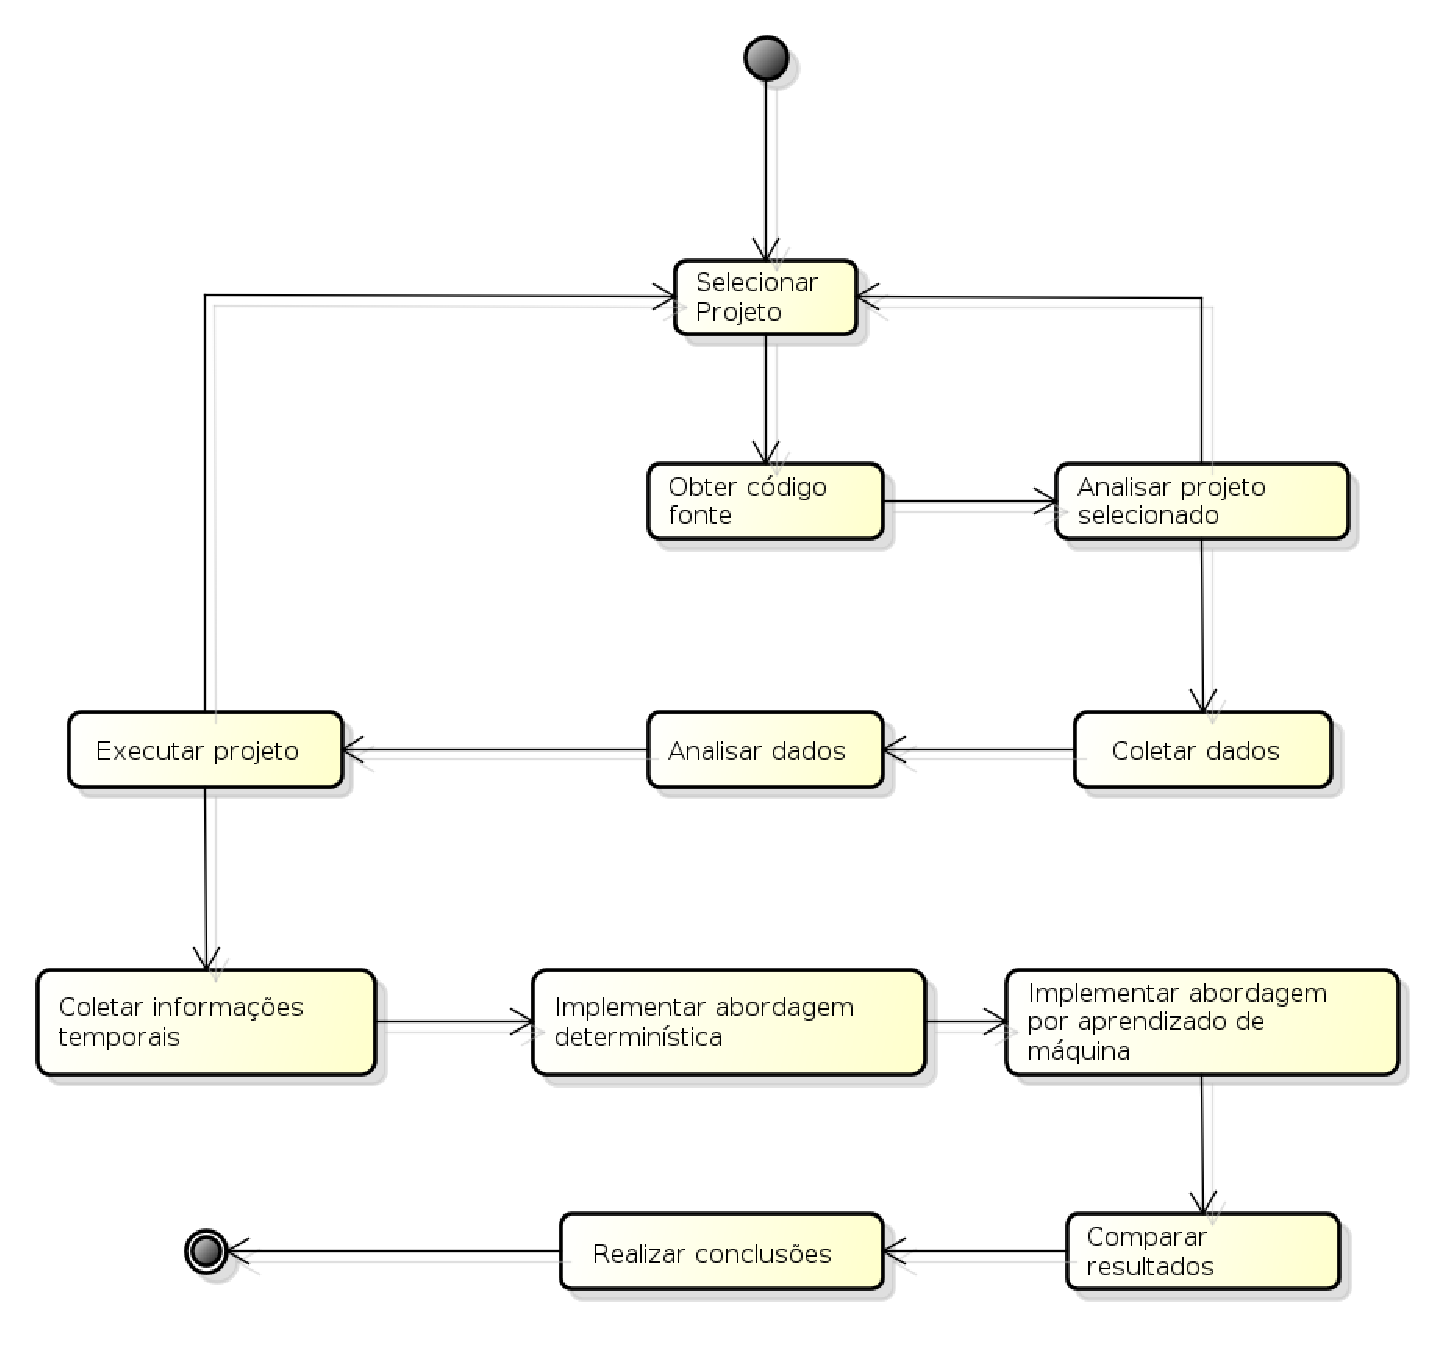
\includegraphics[width=0.9\textwidth]{figuras/planejamento_pesquisa.eps}
  \caption{Processo usando para realização das atividades dessa pesquisa}
  \label{fig:planejamento_pesquisa}
\end{figure}

\begin{enumerate}

    \item \textbf{Selecionar projeto:}
Selecionar um projeto de software livre que implemente um sistema de recomendação baseada em conteúdo e que não leve em consideração questões temporais do pacote quando se realiza tanto
a criação do perfil de usuário e a recomendação propriamente dita. Além disso, deve-se também levar em consideração as dependências do projeto, desde os bibliotecas que depende e os
dados necessitados. Caso o projeto necessite de dados que não possam ser obtidos pelo pesquisadores deste trabalho, o mesmo não poderá ser considerado.

    \item \textbf{Obter código fonte:}
Obter o código fonte do projeto em questão, para que o mesmo possa ser alterado visando o estudo das hipóteses levantadas

    \item \textbf{Analisar projeto selecionado:}
Nesta etapa, o projeto deve ser analisado, visando a compreensão de como o mesmo funciona e, principalmente, os dados necessários para a execução adequada do projeto.

    \item \textbf{Coletar dados:}
Para prover os possíveis dados necessários para o projeto selecionado, uma estratégia de coleta de dados precisa ser definida e implementada.

    \item \textbf{Analisar dados:}
Será necessário analisar os dados coletados, visando descartar dados inválidos e classificar o que foi coletado conforme as necessidades do projeto escolhido.

    \item \textbf{Executar projeto selecionado:}
Com os dados e as dependências do projeto resolvidas, o mesmo deve ser executado, visando encontrar possíveis problemas de execução que não foram previstos e também observar as funcionalidades do projeto.

    \item \textbf{Coletar informações temporais:}
Deve-se implementar uma forma de coletar as informações temporais dos pacotes sendo usados pelo usuário e também prover uma forma de classificar essa informação coletada.

    \item \textbf{Implementar abordagem deterministica:}
Para responder a primeira questão proposta, será necessária implementar uma equação matemática que use as informações de tempo coletadas, juntamente com os outros atributos já usados no projeto selecionado para prover um recomendação.

    \item \textbf{Implementar abordagem por aprendizado de máquina:}
Implementar uma abordagem não-deterministica, no caso uma estratégia de aprendizado de máquina, para usar as informações de tempo coletadas juntamente com os outros atributos providos pelo projeto selecionado para compor um a recomendação.

    \item \textbf{Comparar resultados:}
Para responder as hipóteses propostas será necessário não só comporar as duas
abordagens propostas, determinística e não determinística, e sim comparar ambas
também com as abordagens já implementadas pelo projeto proposto e verificar se
as hipótes se sustentam.

    \item \textbf{Realizar conclusões:}
Com a comparações dos resultados terminada, a mesma deve ser analisada e conclusões devem ser geradas baseada nos fatos apresentados.
\end{enumerate}



\section{Análise dos Dados}

\section{Coleta de dados}

Considerando a necessidade da obtenção dos dados de submissões do
popularity-contest,sistema, foi necessário realizar a coleta dessas submissões
de forma manual. Além de coletar tais informações, decidiu-se coletar algumas
informações adicionais:

\begin{itemize}
    \item \textit{\textbf{Pacotes instalados:}} Necessário para se ter conhecimento dos pacotes que o usuário utiliza;
    \item \textit{\textbf{Pacotes manualmente instalados:}} Estes serão coletados para filtrar as preferências do usuário, para que quando comparado aos pacotes instalados se possa diferenciar pacotes que são automaticamente instalados dos que foram manualmente instalados;
    \item \textit{\textbf{Tempo de acesso e de modificação dos pacotes:}} Estes dados serão usados afim de obter informação quanto a classificação do pacote em relação ao tempo que este foi utilizado;
    \item \textit{\textbf{Caminho do binário de cada pacote:}} Dados coletados afim de se saber qual o binário responsável pela execução do pacote;
    \item \textit{\textbf{Versão do Kernel:}} Necessário para agrupar as recomendações e preferências entre usuários com mesmo kernel;
    \item \textit{\textbf{Distribuição do sistema:}} Necessário para agrupar as recomendações e preferências entre usuários com a mesma distribuição.
    \item \textit{\textbf{Submissão do popularity-contest:}} Informação que é
        utilizada para permitir executar os experimentos de comparação de
        algoritmos.
\end{itemize}

A qualificação da recomendação também será analisada pela coleta de dados
quanto a qual recomendação tem uma maior relevância para o usuário, onde
uma recomendação é o conjunto de pacotes resultantes da execução do
AppRecommender com certos parâmetros definidos. Segue o processo para
coleta da relevância da recomendação para o usuário:

\begin{itemize}
    \item \textit{\textbf{Execução do AppRecommender:}} O AppRecommender é executado várias vezes com parâmetros diferentes, onde cada execução resulta em uma recomendação diferente;
    \item \textit{\textbf{Agrupamento das recomendações:}} Todas as recomendações são agrupadas, ordenadas e são removidas as duplicações de pacotes entre as recomendações;
    \item \textit{\textbf{Pontuação do usuário:}} Para cada pacote no agrupamento das recomendações é solicitado ao usuário que seja dada uma nota de 0 a 10 ao pacote;
    \item \textit{\textbf{Armazenamento das informações:}} É coletado, ou seja, armazenado, cada uma das recomendações, o agrupamento das recomendações e as pontuações de cada pacote.
\end{itemize}

Para armazenar a coleta de dados é criado um diretório na raíz de diretórios
do usuário, onde os dados coletados são
armazenados em arquivos de texto, onde cada arquivo possui o nome de acordo
com o dado que foi coletado e armazenado.


\section{Engenharia de Atributos} \label{engenharia_atributos}

Considerando as limitações da obtenção de dados já discutidas, a pesquisa teve
como objetivo então se focar na recomendação baseada em conteúdo. Dessa forma,
vale a pena detalhar os dados usados para fazer essa recomendação.

Considerando que apenas pacotes Debian podem ser recomendados, os dados sendo
usados atualmente para a realização de uma recomendação podem ser vistos no
arquivo \textit{control} encontrado em qualquer pacote Debian, conforme pode ser
visto na Figura \ref{fig:control_pacote}

\begin{figure}[h]
  \centering
  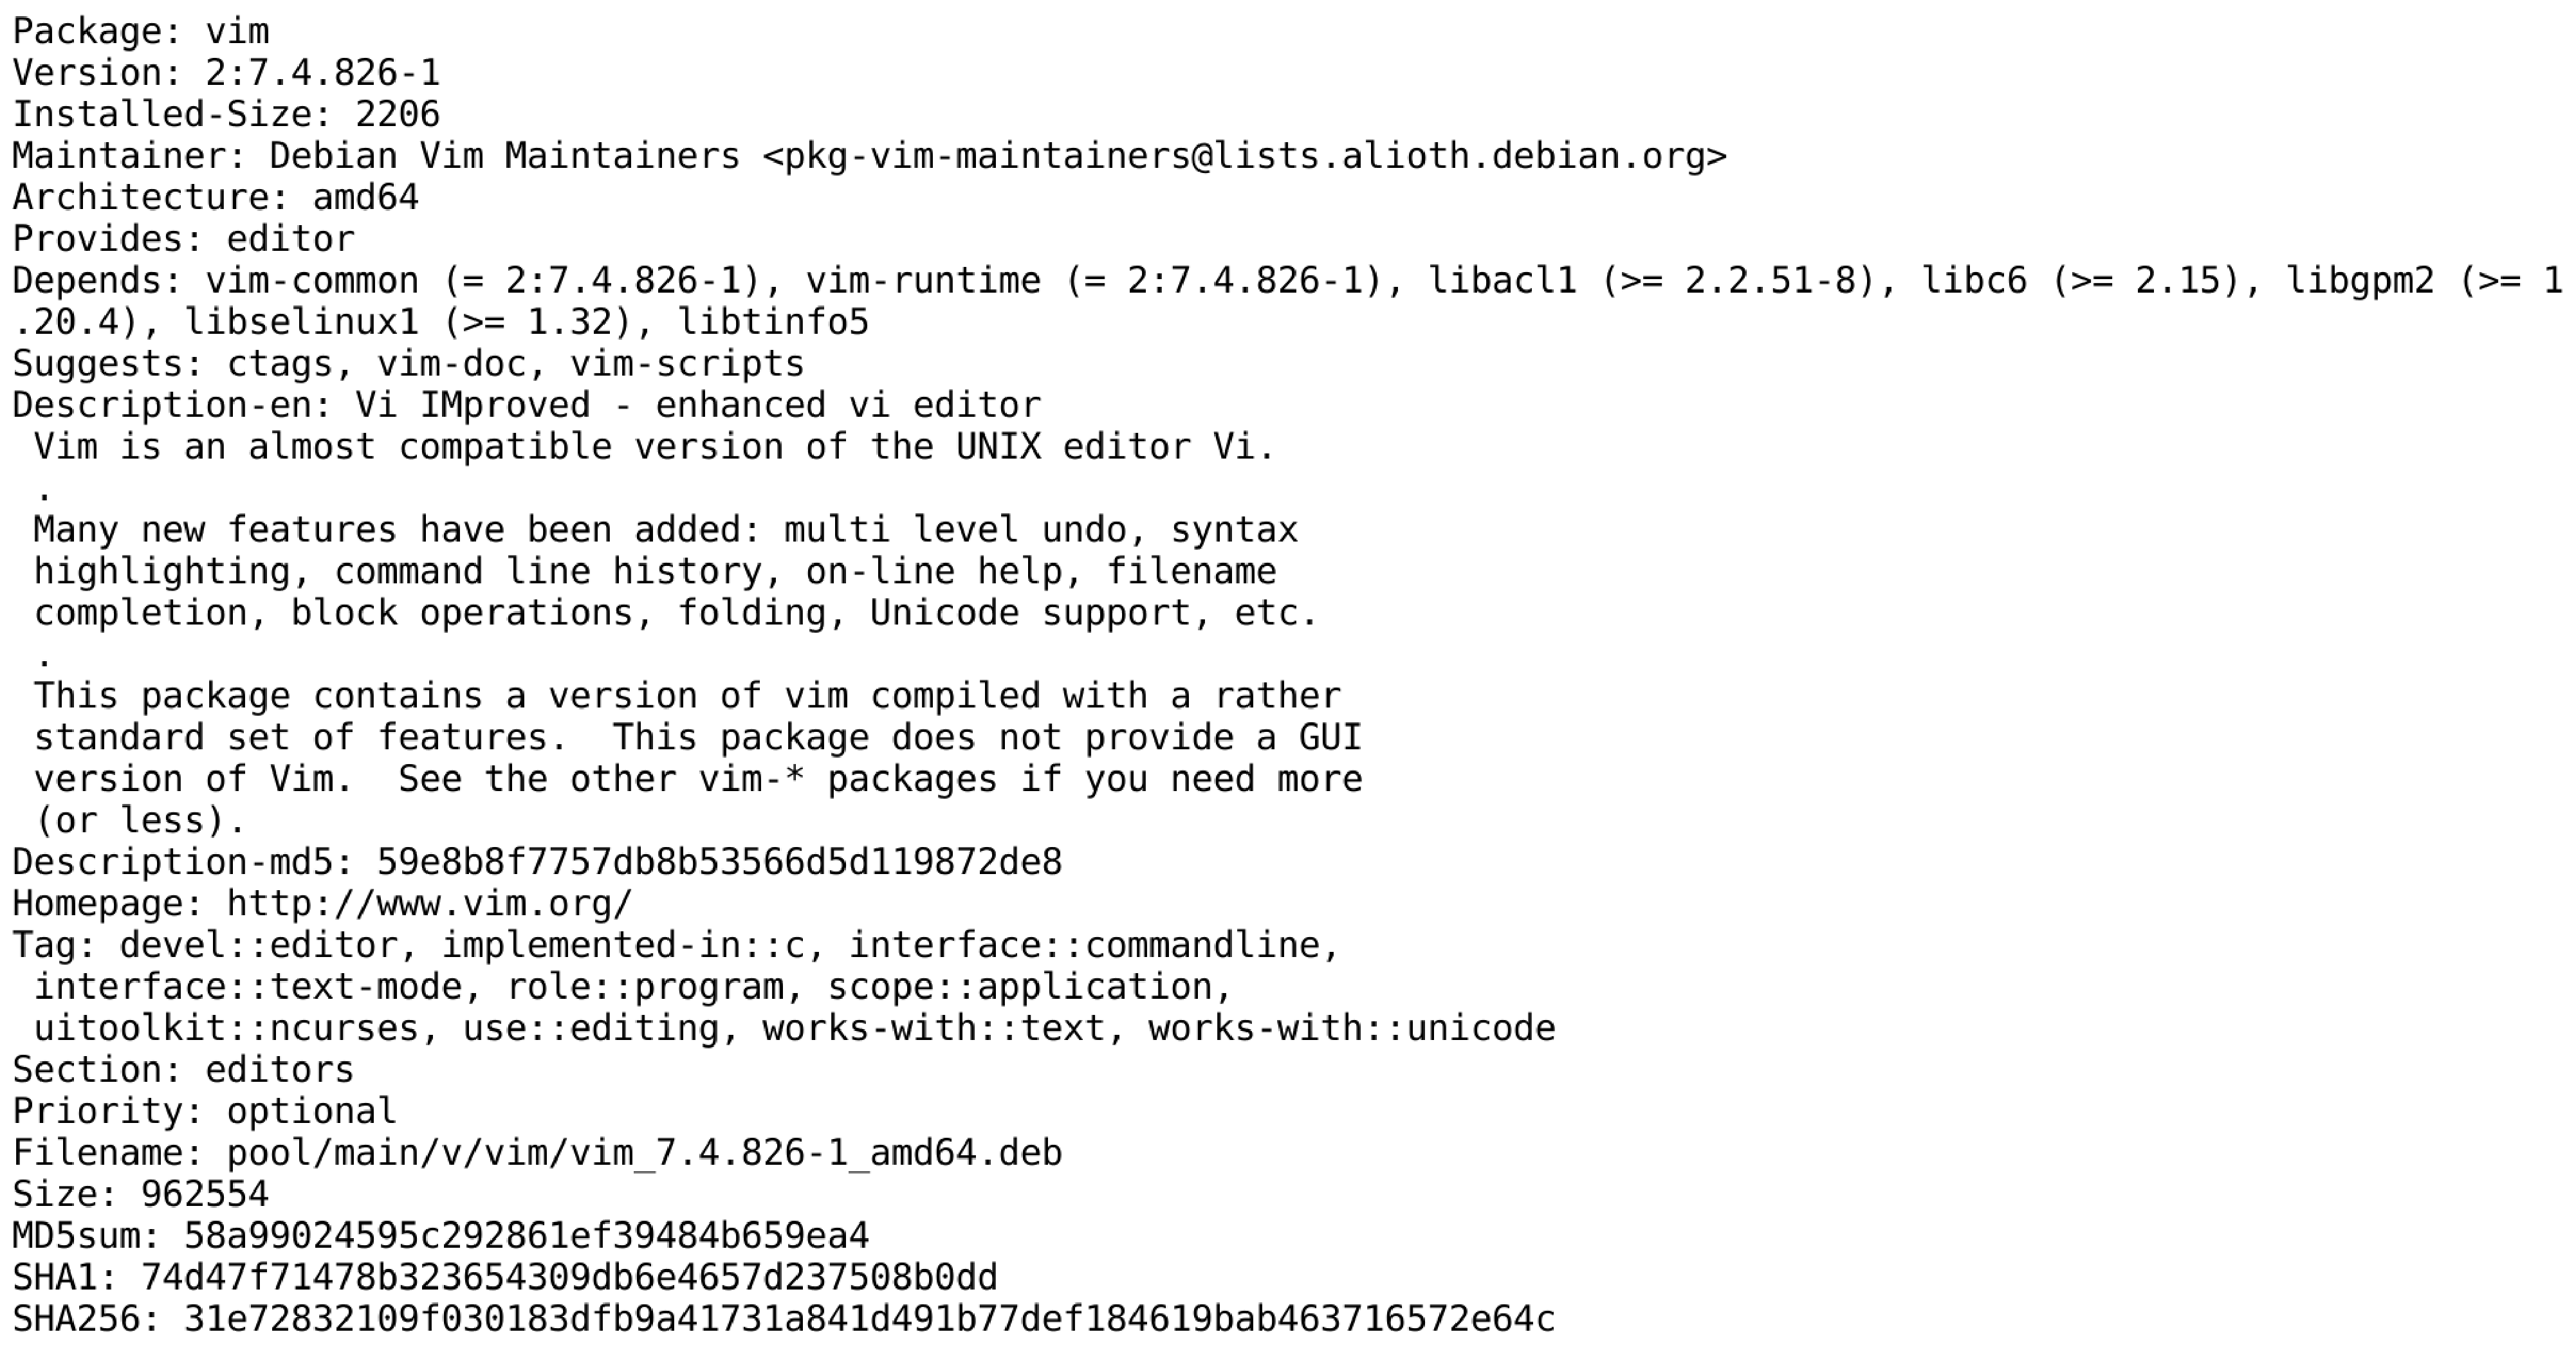
\includegraphics[width=0.9\textwidth]{figuras/control_pacote.eps}
  \caption{Arquivo control de um pacote Debian}
  \label{fig:control_pacote}
\end{figure}

Pode-se ver na Figura \ref{fig:control_pacote} os principais dados usados na
recomendação de um pacote, sendo eles as debtags e a descrição dos pacotes.

As debtags são basicamente um forma de melhor categorizar um pacote fora das 33
seções disponíveis no Debian, além também de permitir que um pacote seja
categorizado em diferentes frentes ao mesmo tempo \cite{zini2005cute}. Isso pode ser visto na Figura
\ref{fig:control_pacote}, onde o software \textit{vim} possui as debtags
\textit{devel::editor} e \textit{interface::commandline}, ou seja, está se
enquadrando tanto como um editor de texto e uma aplicação que roda em linha de
comando.

O processo de criação de debtags é manual, ou seja, um usuário deve associar uma
debtag a um pacote e a comunidade Debian deve verificar se aquela debtag
sugerida condiz com a aplicação em si. Atualmente, existem X pacotes
categorizados com debtags.

Por fim, vale lembrar que nem todas as debtags são consideradas significativas
para o processo de recomendação, sendo que uma filtragem é realizada visando
selecionar apenas as debtags válidas para a construção do perfil do usuário.

A segunda fonte de dado usada é a descrição do pacote, sendo no caso cada termo
individual. A descrição de um pacote é realizada pelo empacotador na hora com
que o mesmo cria o arquivo \textit{control}.

Com essas duas informações, o AppRecommender cria então um perfil de usuário
onde os termos de maior peso são usados para compor tal perfil. Isso é feito por
algoritmos como \textit{Term Frequency Inverse Document Frequency Sub-Linear}
(TFIDF-sublinear) e \textit{Expansão de Query} (ESet).

O perfil de usuário criado é então usado para consultar toda a base de pacotes
do Debian. Isso é realizado através do \textit{apt-xapian-index}, uma aplicação
que provê uma forma de busca pacotes no Debian por meio de Queries, sendo que no
caso do AppRecommender, a query de busca é o perfil gerado para o usuário.
Finalmente, os pacotes retornados são então a recomendação final da aplicação.

Dado esse conjunto de dados, o novo atributo que esta pesquisa pretende
adicionar é o contexto de uso de um pacote, sendo no caso, a última vez que o
mesmo foi usado. Em distribuições Debian, isso pode ser verificado via comando
\textit{stat} o binário do pacote, que tem uma saída que pode ser visualizada na Figura
\ref{fig:comando_stat}.

\begin{figure}[h]
  \centering
  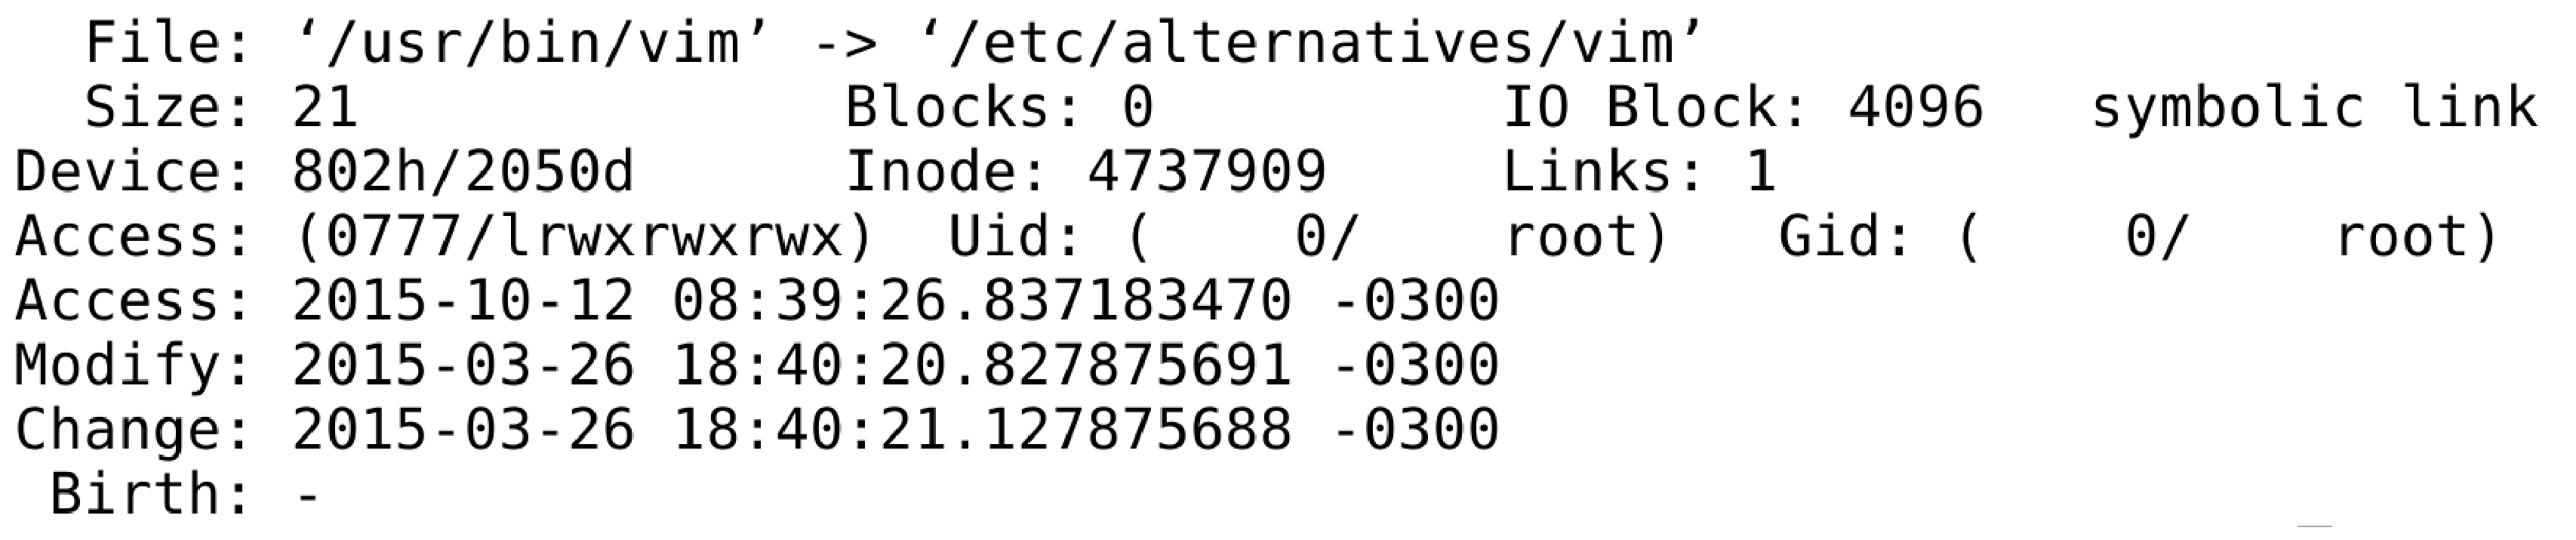
\includegraphics[width=0.9\textwidth]{figuras/comando_stat.eps}
  \caption{Saída do comando \textit{stat} para um dado software}
  \label{fig:comando_stat}
\end{figure}

Pode ser visto na Figura \ref{fig:comando_stat} que o comando exibe os seguintes
atributos de tempo de um dado arquivo \cite{1_haas}:

\begin{itemize}
    \item \textbf{Access:} Última vez que um arquivo foi acessado, ou seja, a
        última vez que seu conteúdo foi de fato acessado.
    \item \textbf{Modify:} Última vez que conteúdo de um arquivo foi modificado.
    \item \textbf{Change:} Última vez que o status de um arquivo foi modificado,
        como mudar as permissões do arquivo e o seu done, ou seja, modificar o
        inode do arquivo.
\end{itemize}

Dessa forma, pode ser visto que o campo \textit{Access} de um arquivo é um dos
principais indicadores de uso de um pacote. Entretanto, o sistema de arquivos
usado pode apresentar uma
restrição neste campo. Isso acontece devido a como o sistema de arquivos é
configurado, pois algumas flags especiais podem ser usadas para alterar como
esse campo é preenchido \cite{2_wiki.debian.org}:

\begin{itemize}
    \item \textbf{noatime:} O sistema de arquivos não irá computar o tempo de
        acesso do arquivo.
    \item \textbf{stricatime:} O sistema de arquivos irá sempre alterar o tempo
        de acesso do arquivo.
    \item \textbf{relatime:} O sistema de arquivos só irá computar o tempo de
        acesso de um arquivo se o valor desse campo for menor que os valores dos
        campos \textit{Modify} e \textit{Change}. Esse opção é default desde
        o kernel 2.6.30, e além disso uma adição foi feita, o tempo de acesso será
        modificado se o mesmo for mais antigo que um dia.
\end{itemize}

O uso do relatime passou a ser default para montar o sistema de arquivos devido
aos problemas de perfomance ocasionados pelo atime. Segundo Ingo Molnar, "atualizar o valor
de atime é de longe uma das maiores deficiências de performance que o Linux possui
hoje" \cite{3_corbet_2007}. Sendo assim, as informações de contexto que serão
usadas, tempo de acesso, modificação e mudança, são aproximações e não
refletem perfeitamente o contexto de uso dos pacotes.

Dessa forma, a informação temporal de cada pacote será obtida pela seguinte
fórmula:

ClassificaçãoTempo = $\frac{TempoAcesso - TempoModificação}{TempoAtual -
TempoModificação}$


Onde:

\begin{itemize}
    \item \textbf{TempoAcesso:} Tempo de último acesso do pacote em segundos.
    \item \textbf{TempoModificação:} Tempo de última modificação do pacote em
        segundos.
    \item \textbf{TempoAtual:} Tempo atual no qual o usuário executa a
        aplicação em segundos.
\end{itemize}


A equação apresentada irá retornar um valor de 0 a 1, sendo que quanto mais
perto de 1, mais recente é considerado o arquivo. Vale ressaltar que a fórmula
também leva em conta o tempo de modificação, pois em algumas situações alterar o
tempo de modificação também altera o tempo de acesso, podendo ocasionar que um
pacote recentemente atualizado tenha um peso menor, pois devido ao fato de que
tanto o tempo de acesso quanto o de modificação são iguais o resultado do
numerador, no calculo da classificação do pacote, será zero

Vale ressaltar que existe uma limitação quanto a essa abordagem, o caso de
pacotes que são executados indiretamente pelo usuário. Existem alguns pacotes
que são executados mesmo sem o usuário necessitar fazer isso manualmente. Dado
este contexto, foi preferível retirar pacotes que apresentam tal comportamento
na hora de selecionar todos os pacotes do usuário.

\section{Teste de hipóteses}

Conforme mencionado na seção \ref{sec:hipoteses}, esta pesquisa se propõem a
criar duas abordagens distintas para prover contexto nas recomendações sendo
feitas. Esta seção irá mostrar como ocorrerá cada abordagem proposta.

\subsection{Abordagem determinística}

A proposta da abordagem determinística é de usar uma fórmula que altere
a criação do perfil de usuário através dos pacotes instalados que foram mais
recentemente usados. A Figura \ref{fig:abordagem_deterministica}
contém o fluxo usado para realizar uma
recomendação utilizando a abordagem determinística.

\begin{figure}[h]
  \centering
  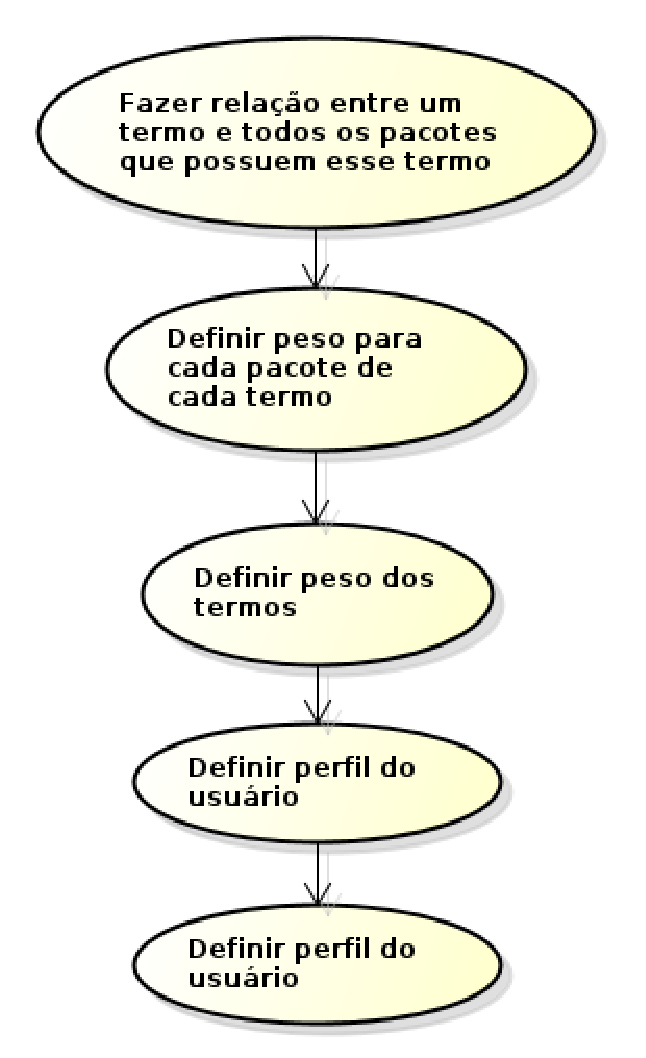
\includegraphics[width=0.9\textwidth]{figuras/abordagem_deterministica.eps}
  \caption{Processo usando para realizar a abordagem deterministica}
  \label{fig:abordagem_deterministica}
\end{figure}

A abordagem determinística é a combinação da estratégia TFIDF combinada com
uma fórmula para adicionar o peso do tempo ao peso calculado pelo TFIDF. Para
isso acontecer, um dicionário associa cada termo, debtag ou palavra da
descrição, aos pacotes onde os mesmos se encontram. Com esse dicionário criado,
no momento que o TFIDF for calculado, o peso temporal do termo também é
calculado e seus valores são enfim multiplicados.

Para calcular o peso temporal de um dado termo, calcula-se primeiro o valor da
classificação no tempo para cada pacote através da fórmula definida na seção
Engenharia de Atributos \ref{sec:engenharia_atributos} para atribuir o valor
a cada um dos pacotes.

Com esse valor calculado, é necessário atribuir mais peso para pacotes que
foram recentemente usados, sendo assim é usado uma função de decaimento
exponencial para obter controle quanto a suavidade da curva que relaciona
a classificação no tempo com o peso do pacote, utilizando a seguinte função:

\textbf{PesoPacote} = C / $\exp\left(({1 - ClassificaçãoTempo}) * {\lambda}\right)$

Onde C e alfa são constantes definidas através de testes realizados na
aplicação, e os valores achados que mais otimizaram a recomendação foram:

\textbf{C} = 1

\textbf{$\lambda$} = 1

Após calcular o peso de cada pacote do termo, o peso to termo é obtido
através da média aritmética dos pesos dos pacotes relacionados ao dado termo.
Com o valor temporal calculado, pode-se enfim multiplicar tal valor com o TFIDF
obtido para o dado termo. Este processo é realizado para todos os termos usados
para se obter o perfil do usuário.

Vale ressaltar que o TFIDF foi usado em relação ao ESet por permitir está fácil
manipulação do peso temporal na construção do perfil no usuário, ao contrário do
algoritmo ESet, onde seria necessário escolher não os termos mais usados, e sim
os pacotes mais recentemente usados para realização da expansão de query. Apesar
de também ser possível utilizar informação temporal neste contexto, foi
preferido utilizar o TFIDF inicialmente, visando entender como cada termo é
priorizado dado a questão temporal proposta.

\subsection{Aprendizado de máquina}

Um dos problemas de se usar apenas a abordagem determinística é uma limitação
encontrada no \textit{apt-xapian-index}, onde não é possível priorizar queries
individuais quando se faz uma busca, por exemplo, dado que na criação do perfil
do usuário, têm-se que o termo "python" apresentou um peso maior que "ruby", mas
ambos os termos estão presentes na query de busca. Quando a busca for realizada,
o peso dos termos será ignorado, tornando os termos equivalentes, mesmo que para
o perfil do usuário eles não o são.

Dessa forma, para a abordagem por aprendizado de máquina, escolheu-se aplicar a
metodologia de filtragem pós-recomendação. Para a projeto em mãos, isso
significa que o mesmo irá continuar fazendo a recomendação conforme foi
desenhado, mas as recomendações serão filtradas pelo perfil de usuário
construído pela abordagem de aprendizado de máquina.

Sendo assim, o enfoque dessa abordagem é usar um algoritmo supervisionado
para criar o perfil do usuário baseado em seus pacotes. Dessa forma, é
necessário definir como cada pacote será apresentado para algoritmo, além de
definir também o valor de cada pacote.

Para o valor do pacote, definiu-se a seguinte escala de classificação baseada na
fórmula proposta na seção de Engenharia de Atributos\ref{engenharia_atributos}:

\begin{table}[h]
\centering
\begin{tabular}{cc}
\hline
\rowcolor[HTML]{EFEFEF}
{Escala} & {Valores} \\ \hline
{Excelent(EX)}  & ClassificaçãoTempo >= 80                  \\ \hline
{Great(G)}   & ClassificaçãoTempo >= 70                  \\ \hline
{Medium(M)}   & ClassificaçãoTempo >= 50                  \\ \hline
{Bad(B)}   & ClassificaçãoTempo >= 30                  \\ \hline
{Horrible(H)}   &ClassificaçãoTempo<30                   \\ \hline
\end{tabular}
\caption{Escala para classificação de um pacote baseado em seus atributos de tempo}
\label{tab:cwe476-erros}
\end{table}


Com a escala definida e as informações de tempo coletadas para cada pacote,
pode-se então criar a classificação de cada pacote manualmente instalado pelo
usuário.
Isso se dá tudo por um script automatizado \footnote{\url{https://github.com/TCC-AppRecommender/AppRecommender/tree/master/src/bin}}
que irá realizar tal função.

Uma vez classificados, os pacotes então podem ser usados como entrada para o
algoritmo supervisionado, visando assim geral o perfil do usuário.
Entretanto, ainda é necessário definir como os dados presentes no pacote serão usados de entrada para o
algoritmo de aprendizado supervisionado. Considerando que os principais dados do pacote sendo usados na
recomendação são as debtags e as palavras que compõem sua descrição, escolheu-se usar uma abordagem de
vetor binário para cada um dos items. Sendo assim, os vetor de entrada será composto pela agregação de dois vetores
binários.

Para as debtags, o vetor binário irá ter o tamanho igual ao número de debtags
válidas definidas pelo AppRecommeder, sendo no caso 276 debtags. Sendo assim, o
vetor binário irá representar as debtags ordenadas em ordem alfabética. Dessa forma,
o vetor binário de um dado pacote irá conter o valor "0" caso o mesmo não contenha uma debtag e "1" caso a mesma se encontre
no pacote. Por exemplo, dado um conjunto de três debtags role:program, implemented-in:c e devel:editor, e um pacote com a debtag
role:program associado a ele, o seu vetor binário seria o seguinte: [0, 0, 1].

Para os termos da descrição, a formatação do vetor é um pouco diferente. Primeiramente, optou-se por usar os termos apenas presentes
nos pacotes manualmente instalados do usuário e não no banco de dados do Debian. Isso se dá para reduzir o tamanho do vetor e também
pelo fato de que se um termo não aparece em nenhum pacote instalado pelo usuário, o mesmo em tese não terá nenhum peso relevante na
classificação. Além disso, foi necessário retirar termos comuns do vetor de termos produzido, como por exemplo os termos "a" e "the" que
aparecem em praticamente todo pacote mas não representam nenhuma vantagem na hora de avaliar um pacote. Uma vez gerado o vetor de todos os
termos dos pacotes do usuário e aplicar o filtro de termos comuns, a abordagem de vetor binário pode ser usada, funcionando de forma
similar ao vetor binário das debtags, onde os termos estarão representados em ordem alfabética e caso o pacote contenha tal termo em sua
descrição, a posição do vetor associado ao termo será marcada como "1".

Com a combinação desses valores, chega-se então a forma final da entrada de um pacote para o uso de algoritmos de aprendizado
supervisionados. Observa-se também que para propósitos de armazenamento, a classificação do pacote também é armazenada ao final da combinação
dos vetores binários dos termos e debtags. A Figura X mostra a versão final da formatação de dados de um pacote:

OBS: Imagem ainda não incluída pois o vetor binário dos termos ainda não está
sendo filtrado, gerando assim um vetor muito grande para caber em uma imagem.

Por fim, os pacotes então podem finalmente ser usados para alimentar o algoritmo de aprendizado escolhido para a pesquisa, sendo no caso um
classificador bayesiano. A escolha desse classe de algoritmo se deu por alguns fatores. O primeiro se dá pela popularidade do algoritmo para
sistemas de recomendação por conteúdo \cite{amatriain2011data}. Outro fator que levou a escolha desse algoritmo é a sua capacidade de produzir
modelos eficazes sem necessitar um enorme processamento de dados, além do fato
de que o modelo gerado é facilmente compreensível, diferente de outros métodos,
como redes neurais\cite{segaran2007programming}.

Vale ressaltar também que algoritmos de aprendizado supervisionados não-lineares foram considerados, como redes neurais. Entretanto, segundo
a pesquisa realizada por \cite{pazzani1997learning} o uso de redes neurais em relação ao classificador bayesiano não mostra nenhuma melhoria
considerável para sistema de recomendação. Sendo assim, optou-se por usar o classificador bayesiano de início e caso o modelo não apresente
resultados satisfatórios, mudar então para um algoritmo supervisionado não-linear.

É importante também ressaltar que o algoritmo será validado não só pela técnicas usadas no AppRecommender, mas também técnicas próprias de
aprendizado de máquina serão usadas para verificar se o modelo gerado está satisfatório, como a validação cruzada, sendo o foco principal a
identificação de \textit{overfitting} e \textit{underfitting}.

Com o perfil de usuário criado e validado, toda vez que uma recomendação for gerada, os pacotes escolhidos serão filtrados pelo perfil criado,
sendo que apenas os pacotes classificados com EX ou G serão qualificados para a recomendação ao usuário.
